\chapter{Avaliação Experimental do Sistema de Controle}\label{cap6}
Após projetar os controladores faremos uma avaliação do seu funcionamento aplicando cada um no sistema real.
\section{Descrição e objetivos experimentais}
Os experimentos descritos neste capítulo tem como objetivo verificar e avaliar o funcionamento do sistema ao ser controlado pelos controladores projetados no capítulo \ref{cap5}. Serão executados 4 experimentos no sistema que funcionam da seguinte forma:
\paragraph{Resposta ao Degrau Unitário} A resposta ao degrau unitário é um experimento onde o sistema recebe uma referência unitária e reage à ela. Com este experimento iremos verificar se o sistema se mantém estável ao ser controlado e se ele atende aos requisitos definidos quando o controlador foi projetado.
\paragraph{Resposta à escadaria} A resposta à escadaria é um experimento onde o sistema recebe alguns níveis de referência ao longo do tempo e medimos sua resposta para ver como reage à mudança de referência.

\paragraph{Teste de Robustez à Mudança de Parâmetros}

O teste de robustez à mudança de parâmetros serve para determinar se o controlador é capaz de reagir quando algum parâmetro é alterado. Neste experimento alteramos o peso da bola e verificamos se o sistema mantém a referência.

\paragraph{Teste de Robustez à Perturbação Externa}
  O teste de robustez à perturbação externa mostra se o sistema controlado é capaz de rejeitar perturbações externas ao sistema. Para executar este teste iremos medir a resposta do sistema enquanto obstruímos a saída de ar através dos buracos inferiores do duto do túnel de vento, efetivamente aumentando o fluxo de ar que eleva a bola.

\section{Resultados Experimentais}
Nesta seção serão apresentados os resultados dos experimentos descritos anteriormente.
\subsection{Resultados da Resposta ao degrau unitário}\label{rstep}

\begin{figure}[H]
	\centering
	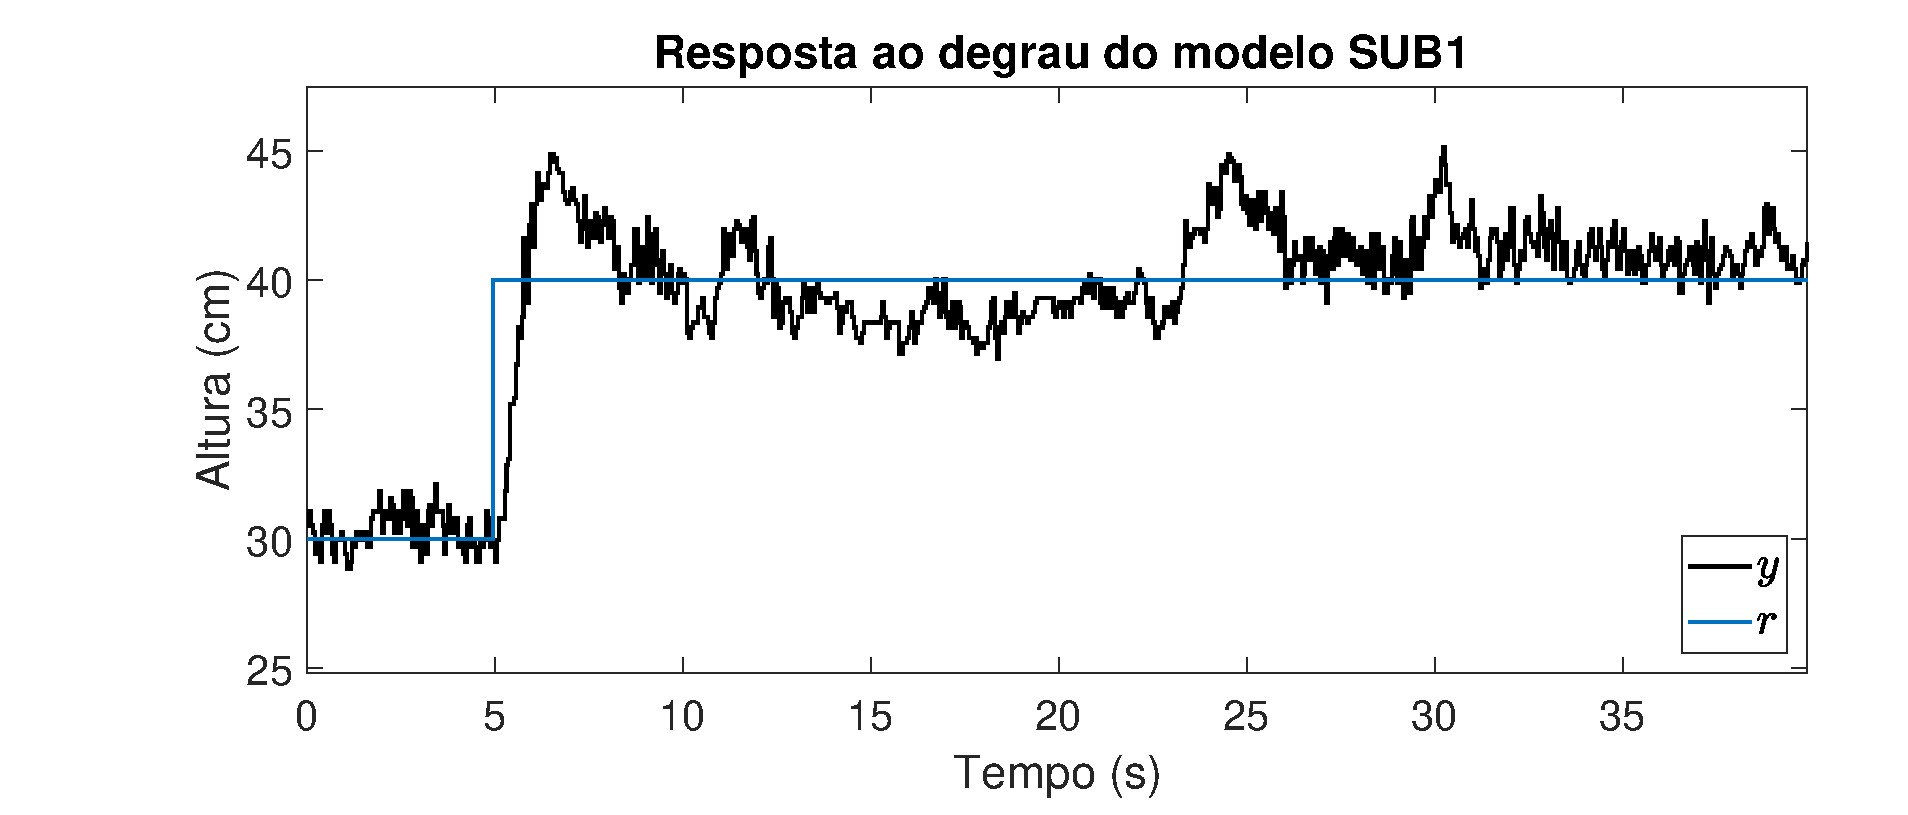
\includegraphics[width=1\linewidth]{steprealsub1}
	\caption[Resposta ao degrau do sistema controlado $SUB1$]{Resposta ao degrau do sistema usando o controlador $SUB1$}
	\label{fig:steprealsub1}
\end{figure}

\begin{figure}[H]
	\centering
	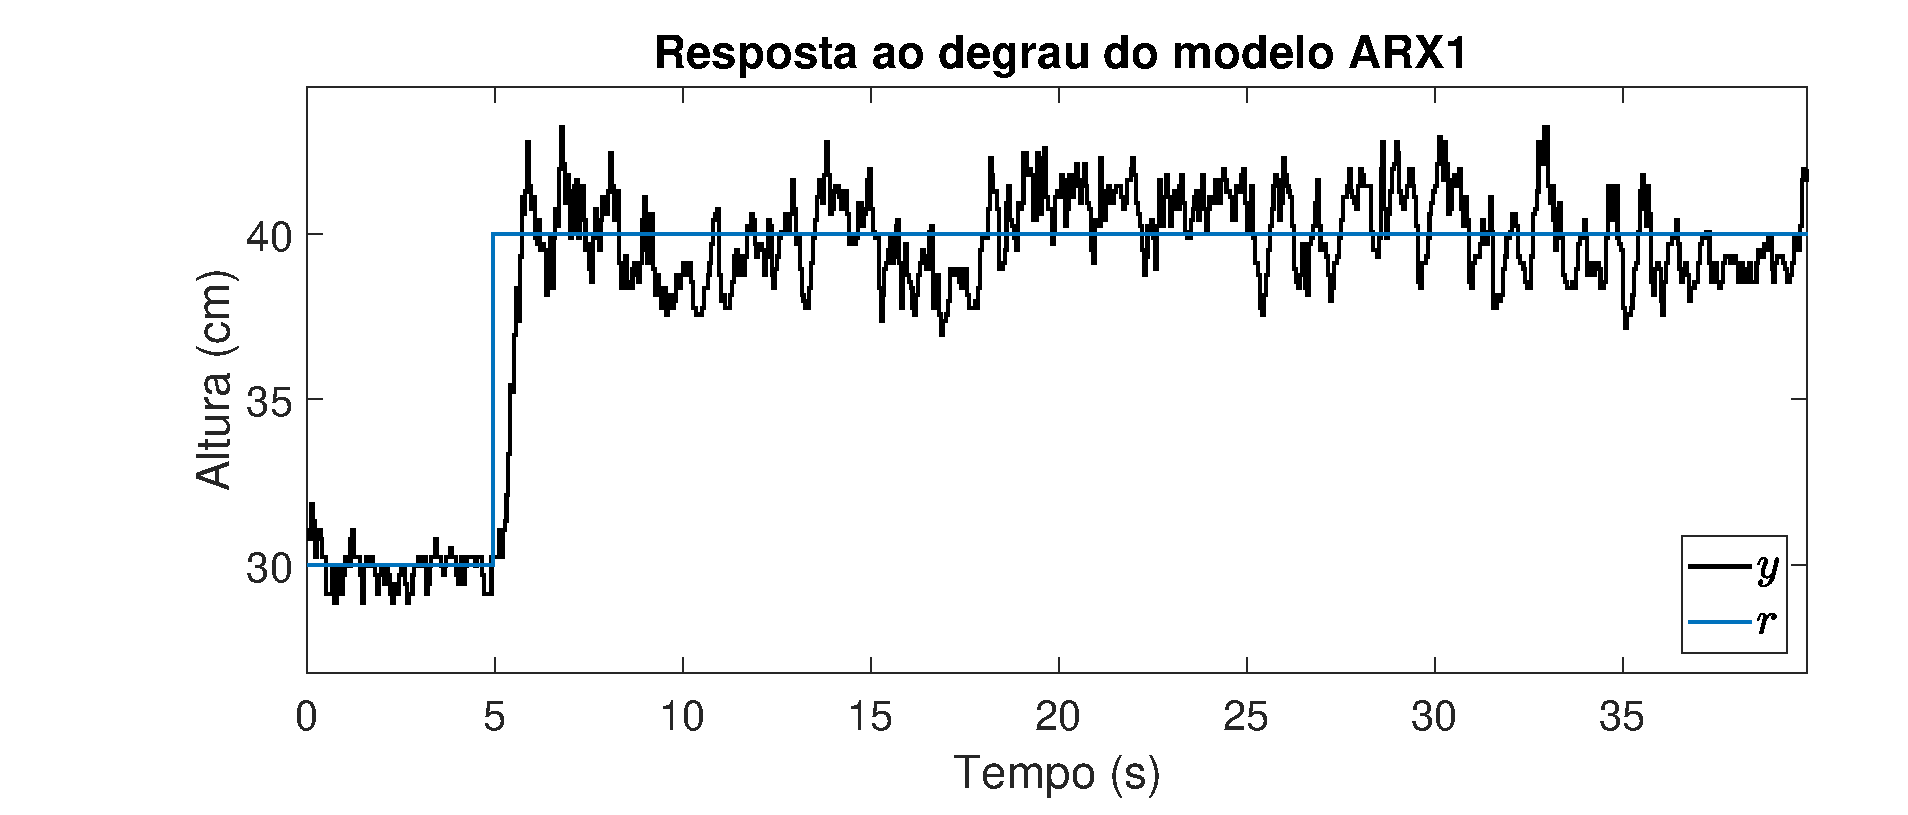
\includegraphics[width=1\linewidth]{steprealarx1}
	\caption[Resposta ao degrau do sistema controlado $ARX1$]{Resposta ao degrau do sistema usando o controlador $ARX1$}
	\label{fig:steprealarx1}
\end{figure}

\begin{figure}[H]
	\centering
	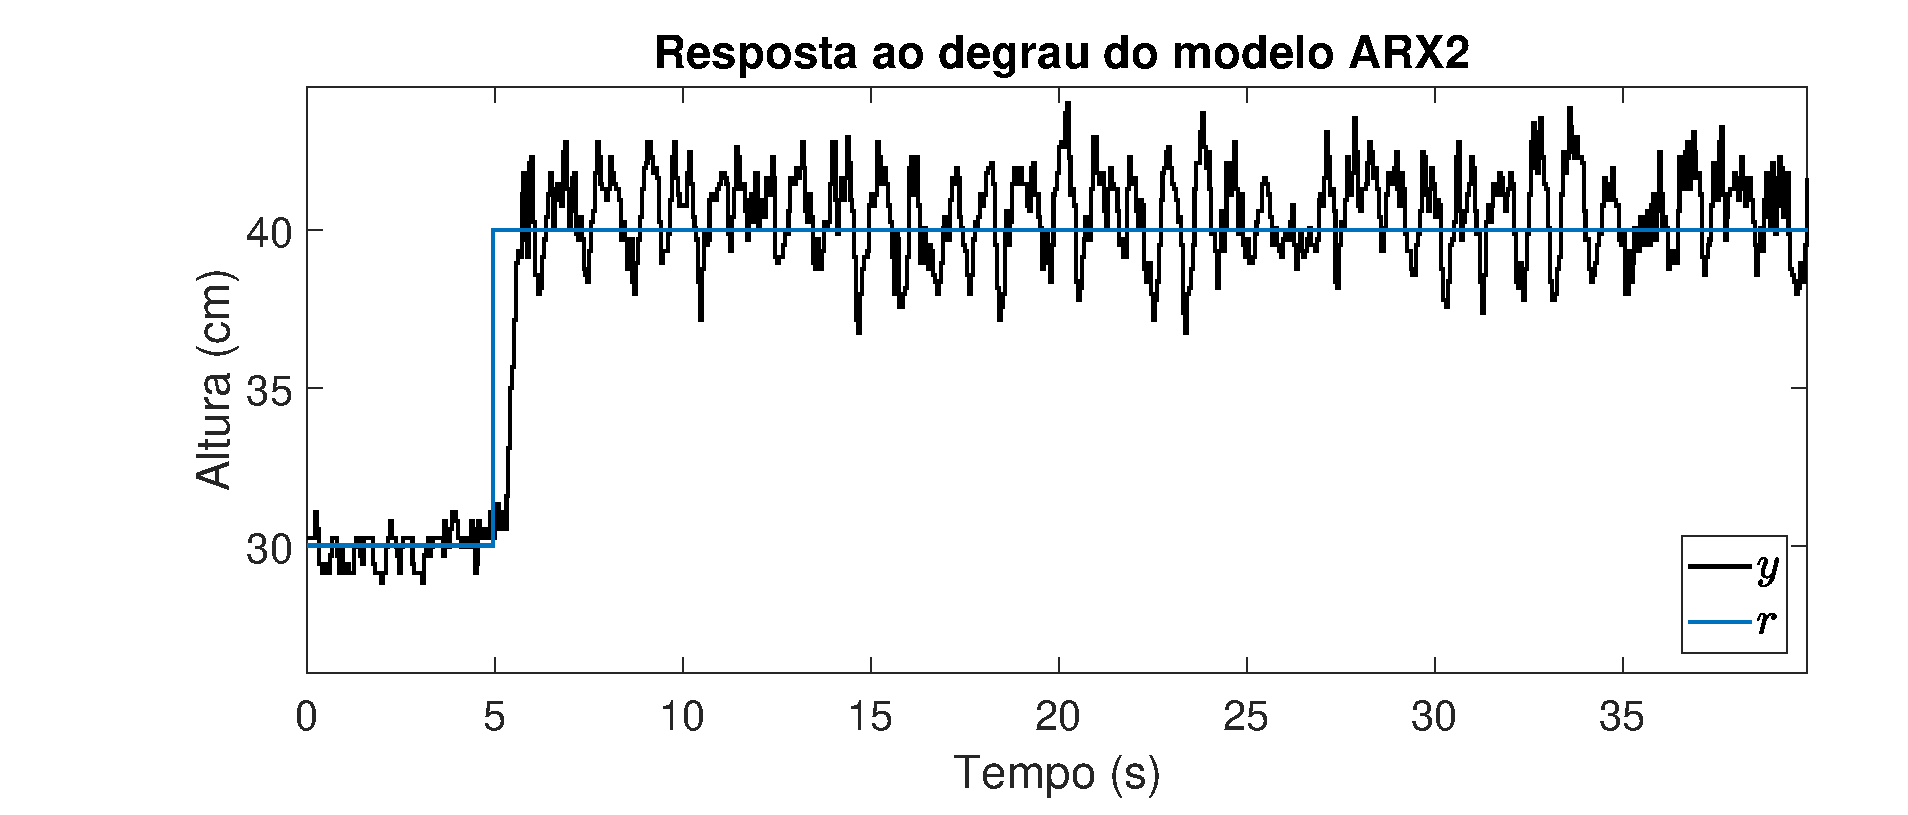
\includegraphics[width=1\linewidth]{steprealarx2}
	\caption[Resposta ao degrau do sistema controlado $AR21$]{Resposta ao degrau do sistema usando o controlador $ARX2$}
	\label{fig:steprealarx2}
\end{figure}

\subsection{Resultados da Resposta à escadaria}\label{rstair}

\begin{figure}[H]
	\centering
	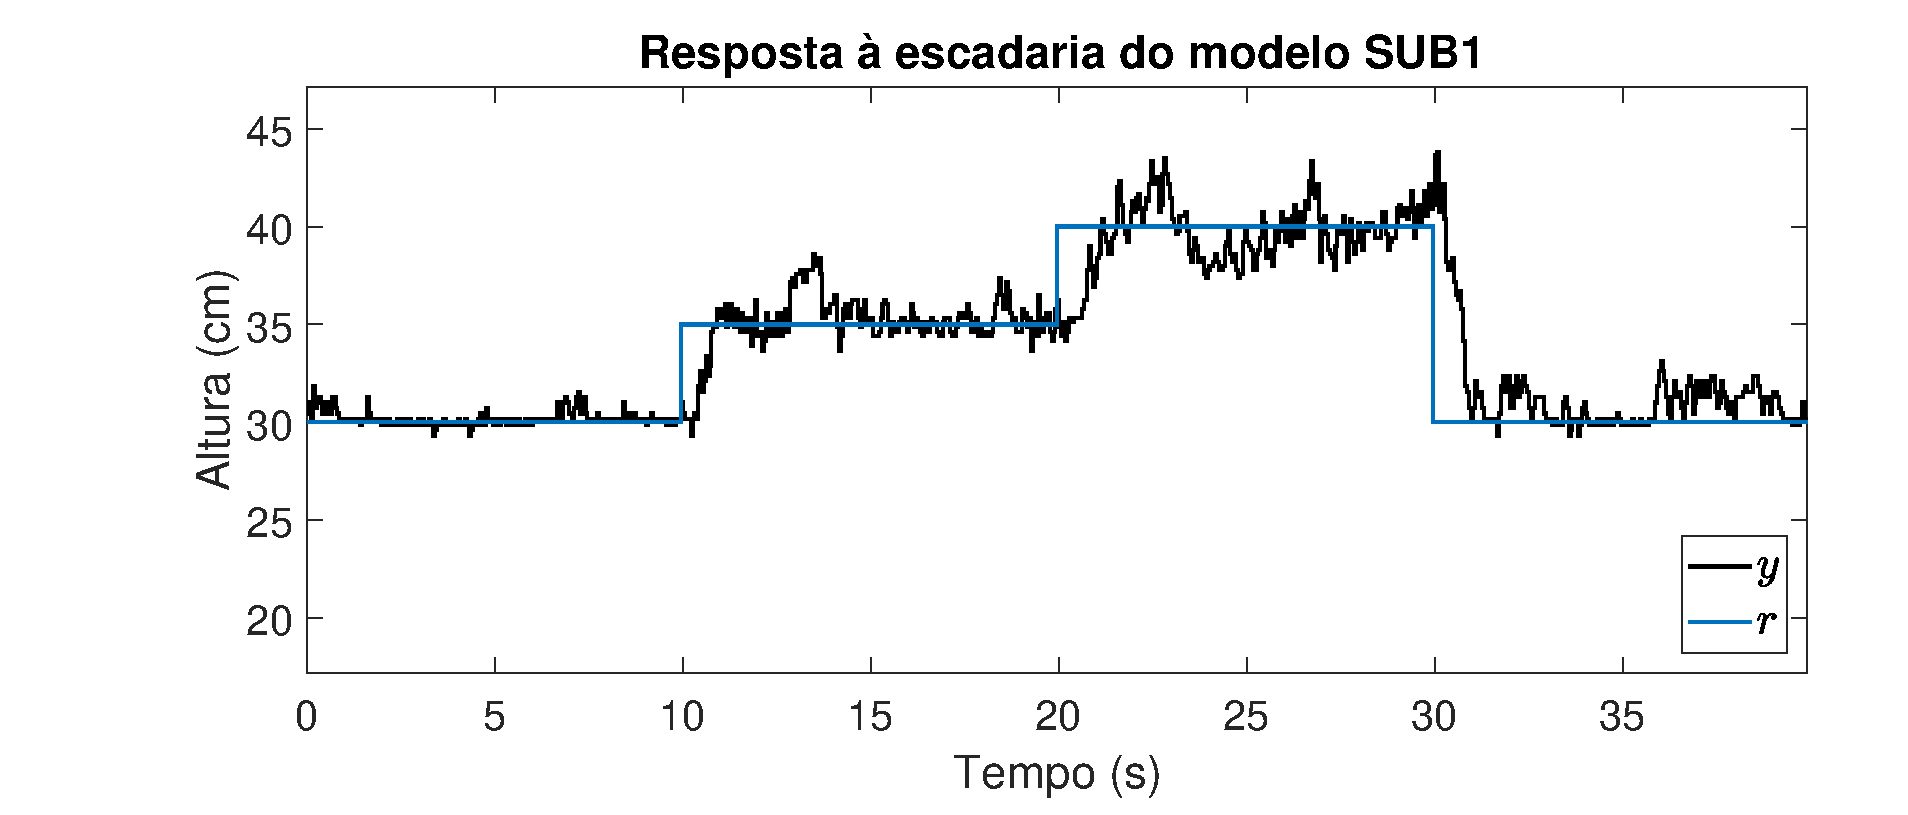
\includegraphics[width=1\linewidth]{stairrealsub1}
	\caption[Resposta à escadaria do sistema controlado $SUB1$]{Resposta à escadaria do sistema usando o controlador $SUB1$}
	\label{fig:stairrealsub1}
\end{figure}

\begin{figure}[H]
	\centering
	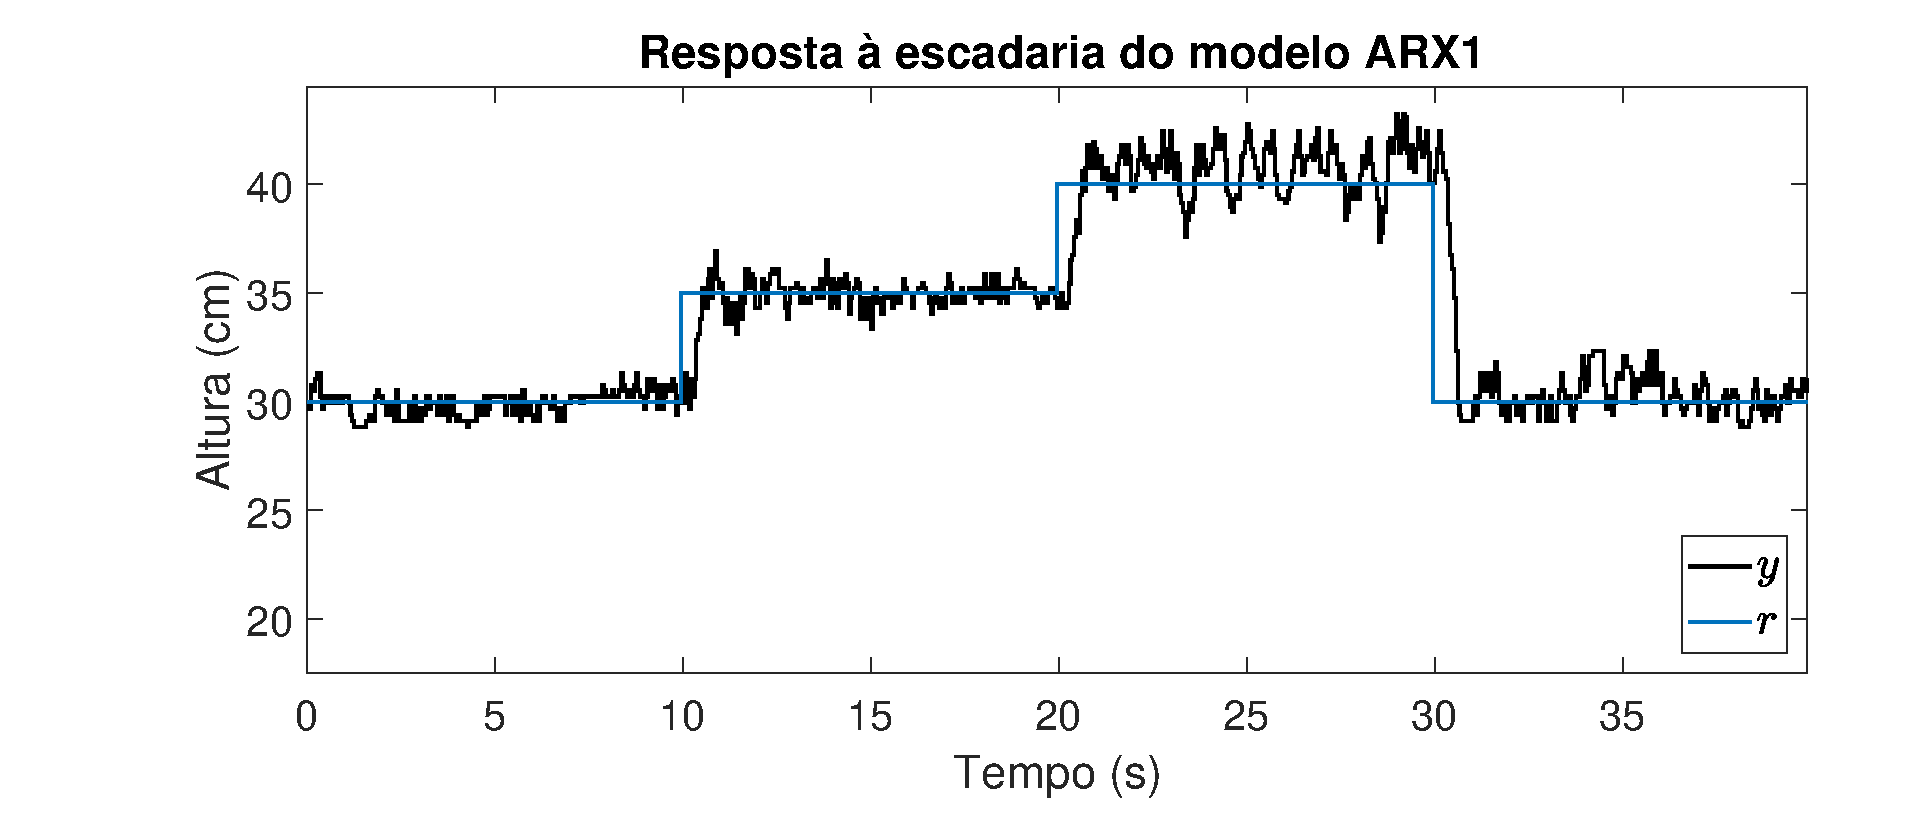
\includegraphics[width=1\linewidth]{stairrealarx1}
	\caption[Resposta à escadaria do sistema controlado $ARX1$]{Resposta à escadaria do sistema usando o controlador $ARX1$}
	\label{fig:stairrealarx1}
\end{figure}

\begin{figure}[H]
	\centering
	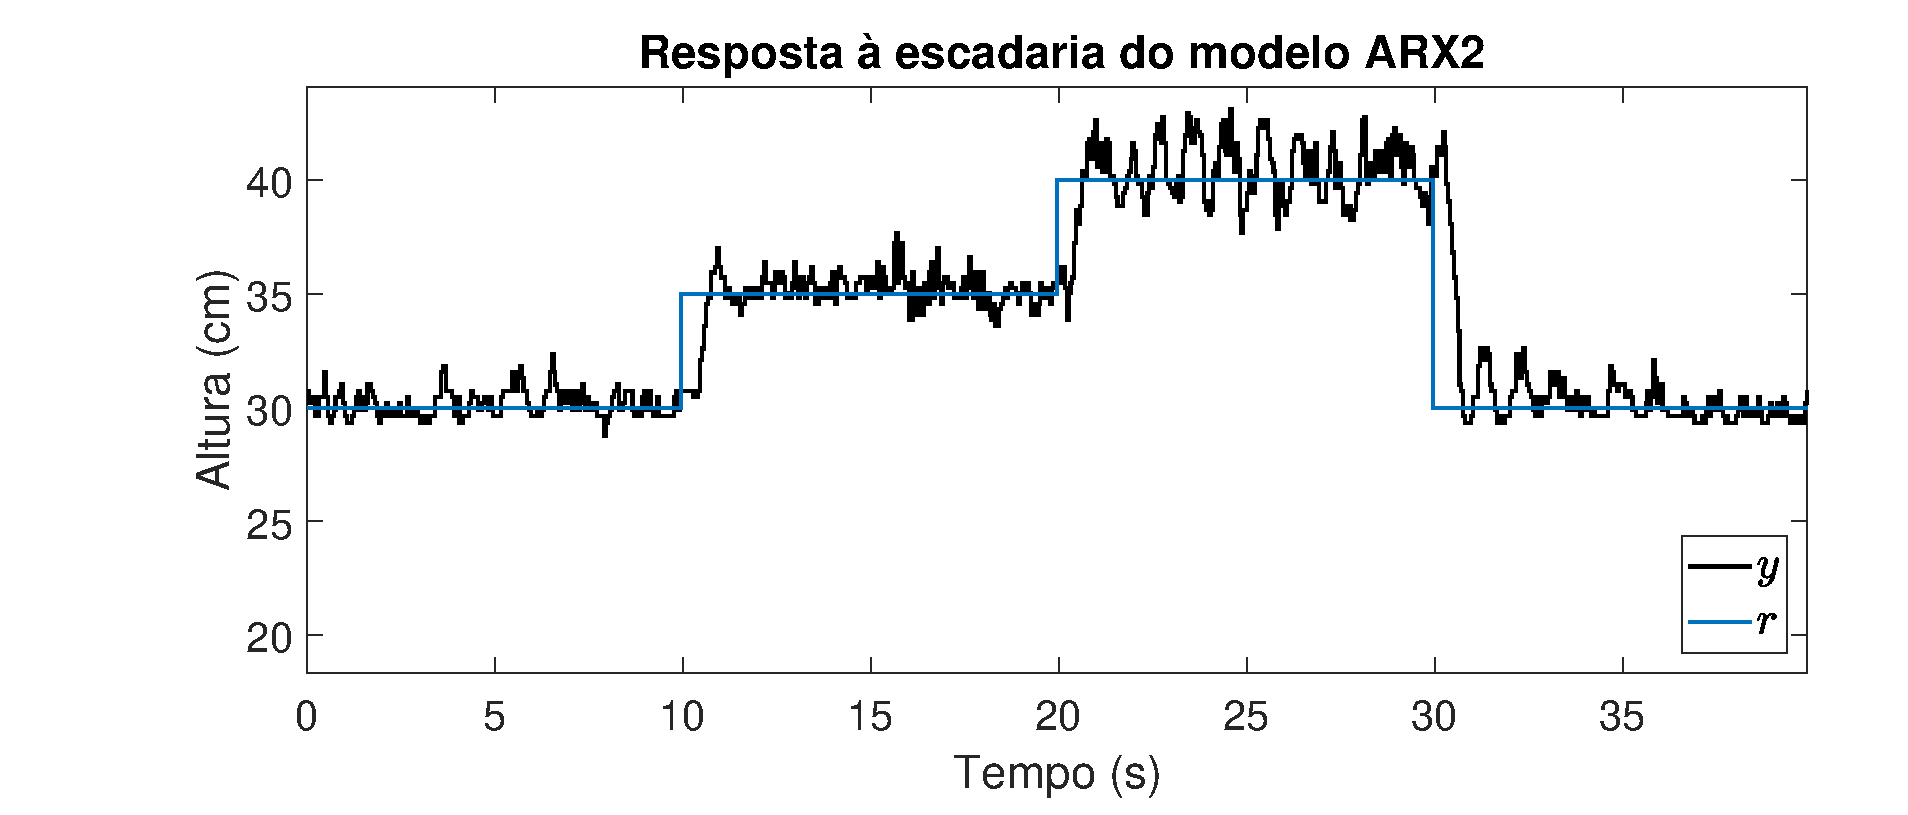
\includegraphics[width=1\linewidth]{stairrealarx2}
	\caption[Resposta à escadaria do sistema controlado $ARX2$]{Resposta à escadaria do sistema usando o controlador $ARX2$}
	\label{fig:stairrealarx2}
\end{figure}

\subsection{Resultados do Teste de Robustez à mudança de Parâmetros}\label{rmp}

\begin{figure}[H]
	\centering
	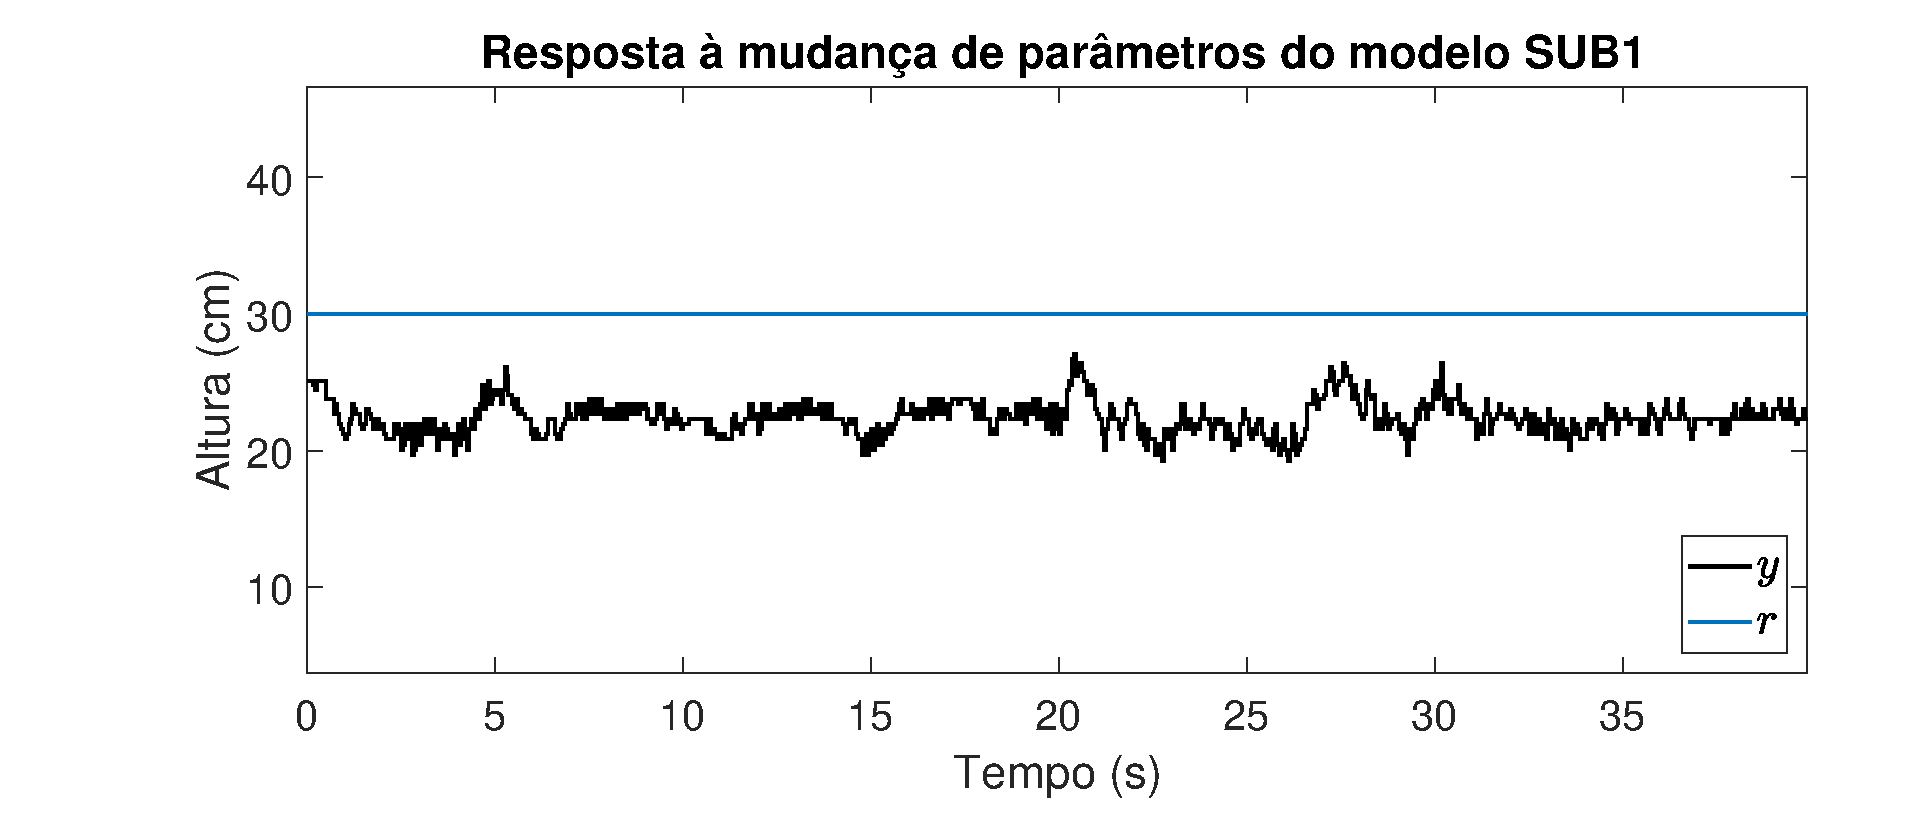
\includegraphics[width=1\linewidth]{mprealsub1}
	\caption[Resposta à mudança de parâmetros do modelo $SUB1$]{Resposta à mudança de parâmetros do sistema com o controlador do modelo $SUB1$}
	\label{fig:mprealsub1}
\end{figure}

\begin{figure}[H]
	\centering
	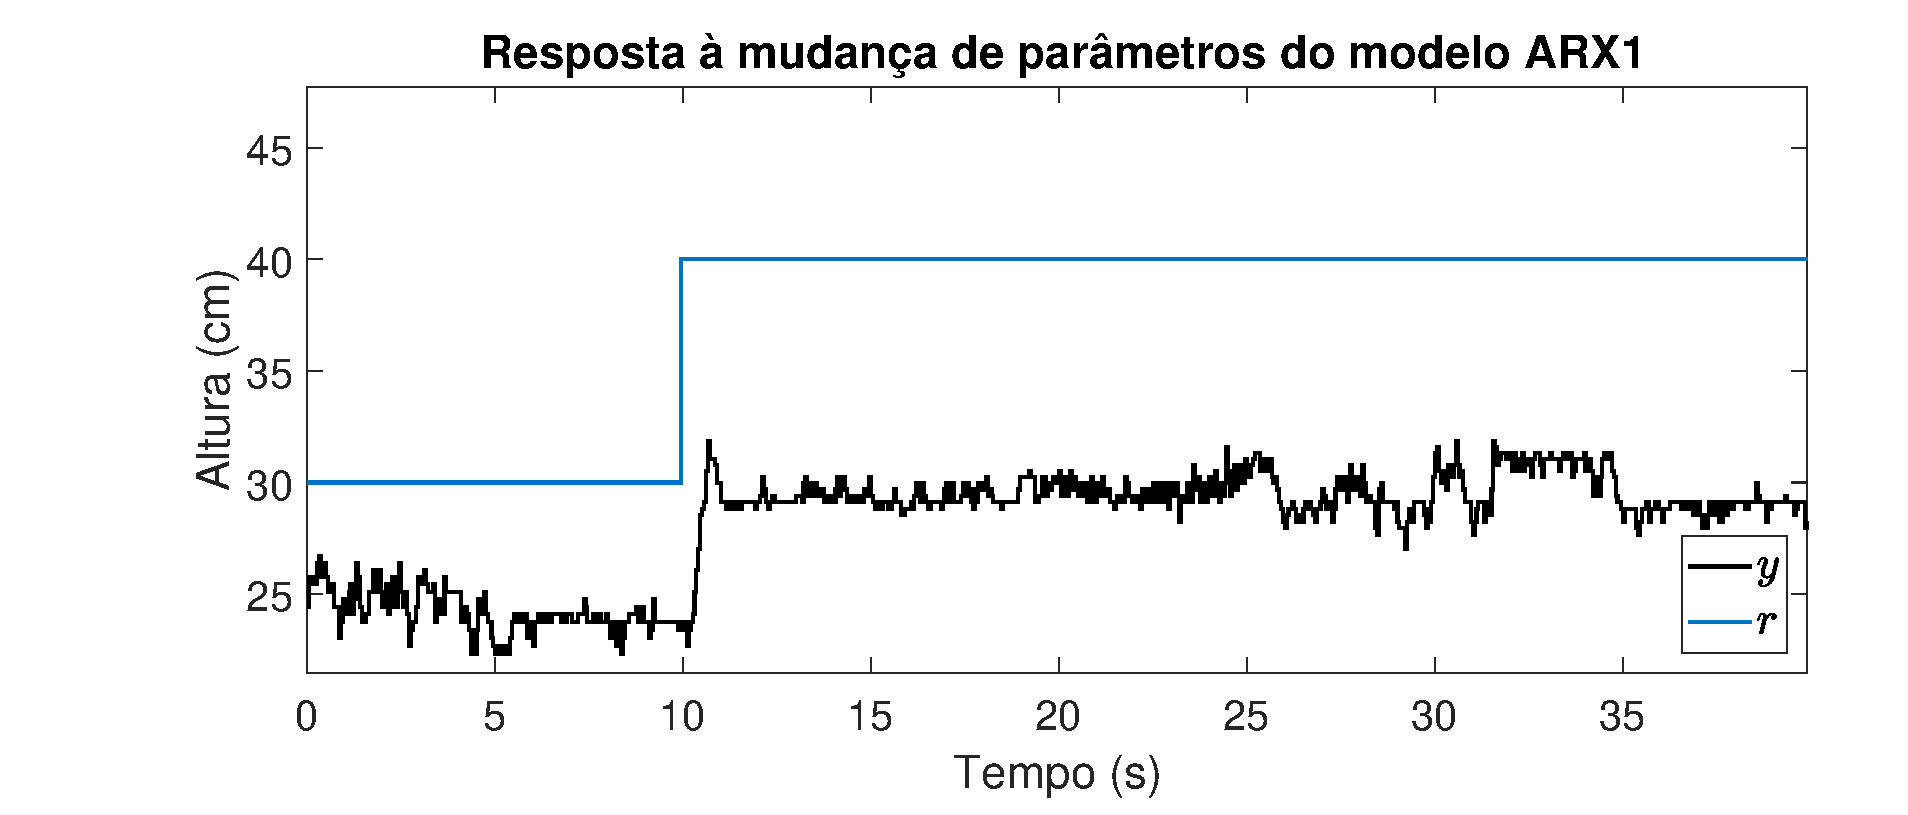
\includegraphics[width=1\linewidth]{mprealarx1}
	\caption[Resposta à mudança de parâmetros do modelo $ARX1$]{Resposta à mudança de parâmetros do sistema com o controlador do modelo $ARX1$}
	\label{fig:mprealarx1}
\end{figure}

\begin{figure}[H]
	\centering
	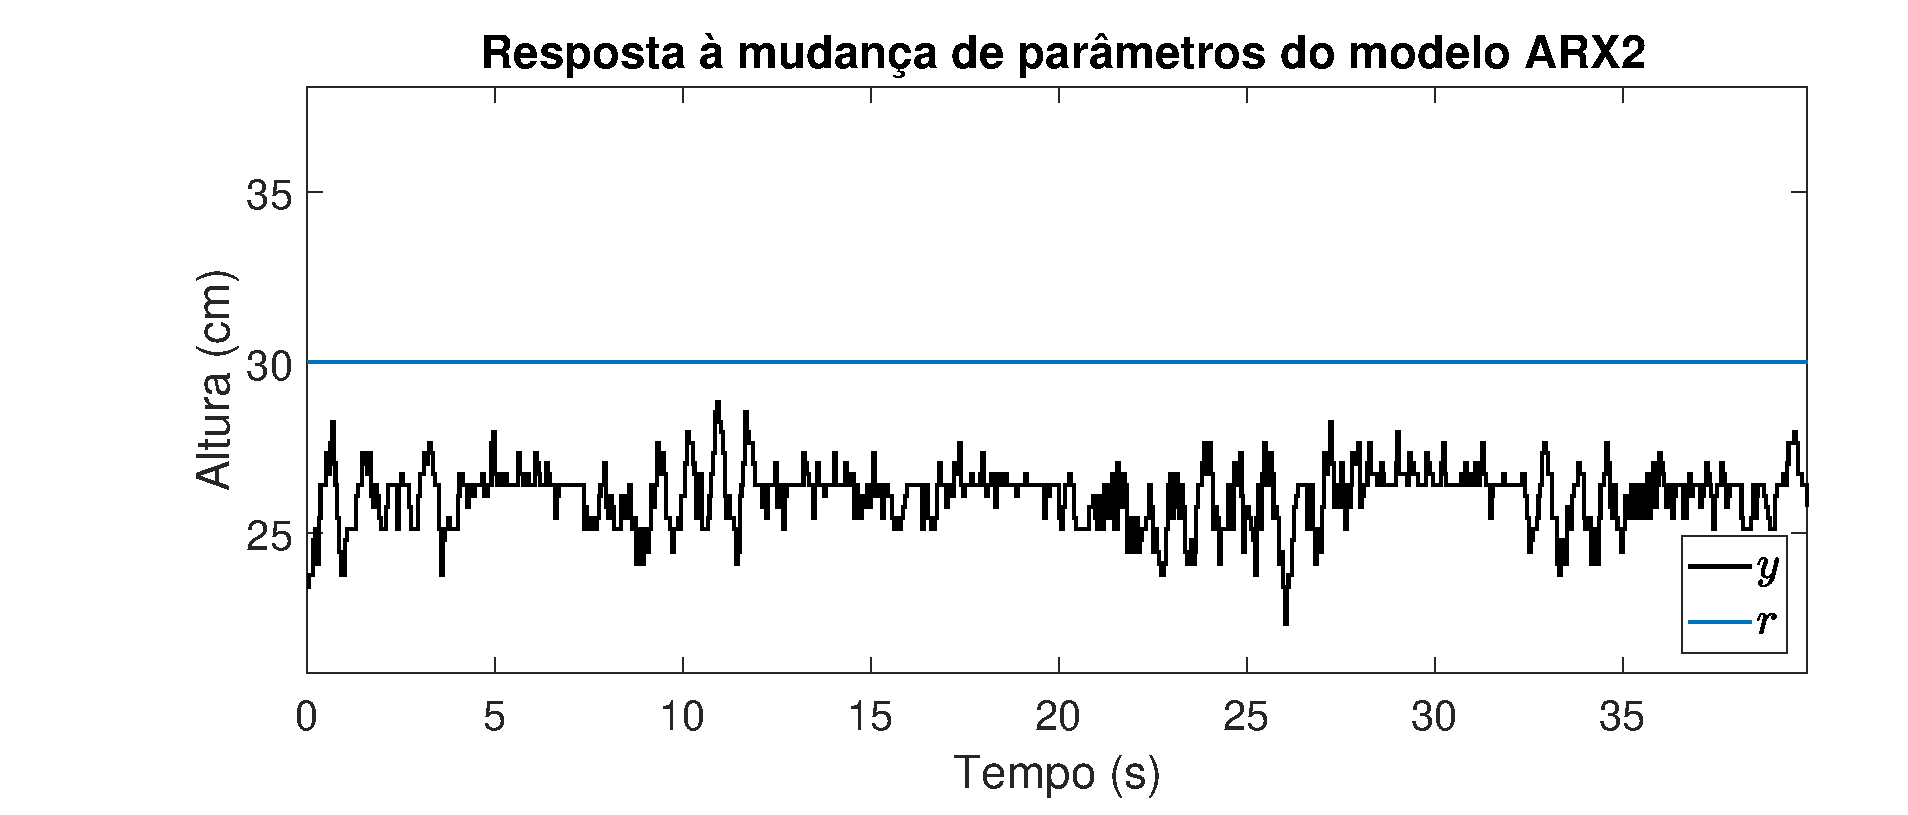
\includegraphics[width=1\linewidth]{mprealarx2}
	\caption[Resposta à mudança de parâmetros do modelo $ARX2$]{Resposta à mudança de parâmetros do sistema com o controlador do modelo $ARX2$}
	\label{fig:mprealarx2}
\end{figure}


\subsection{Resultados do Teste de Robustez à perturbação externa}\label{rpe}

\begin{figure}[H]
	\centering
	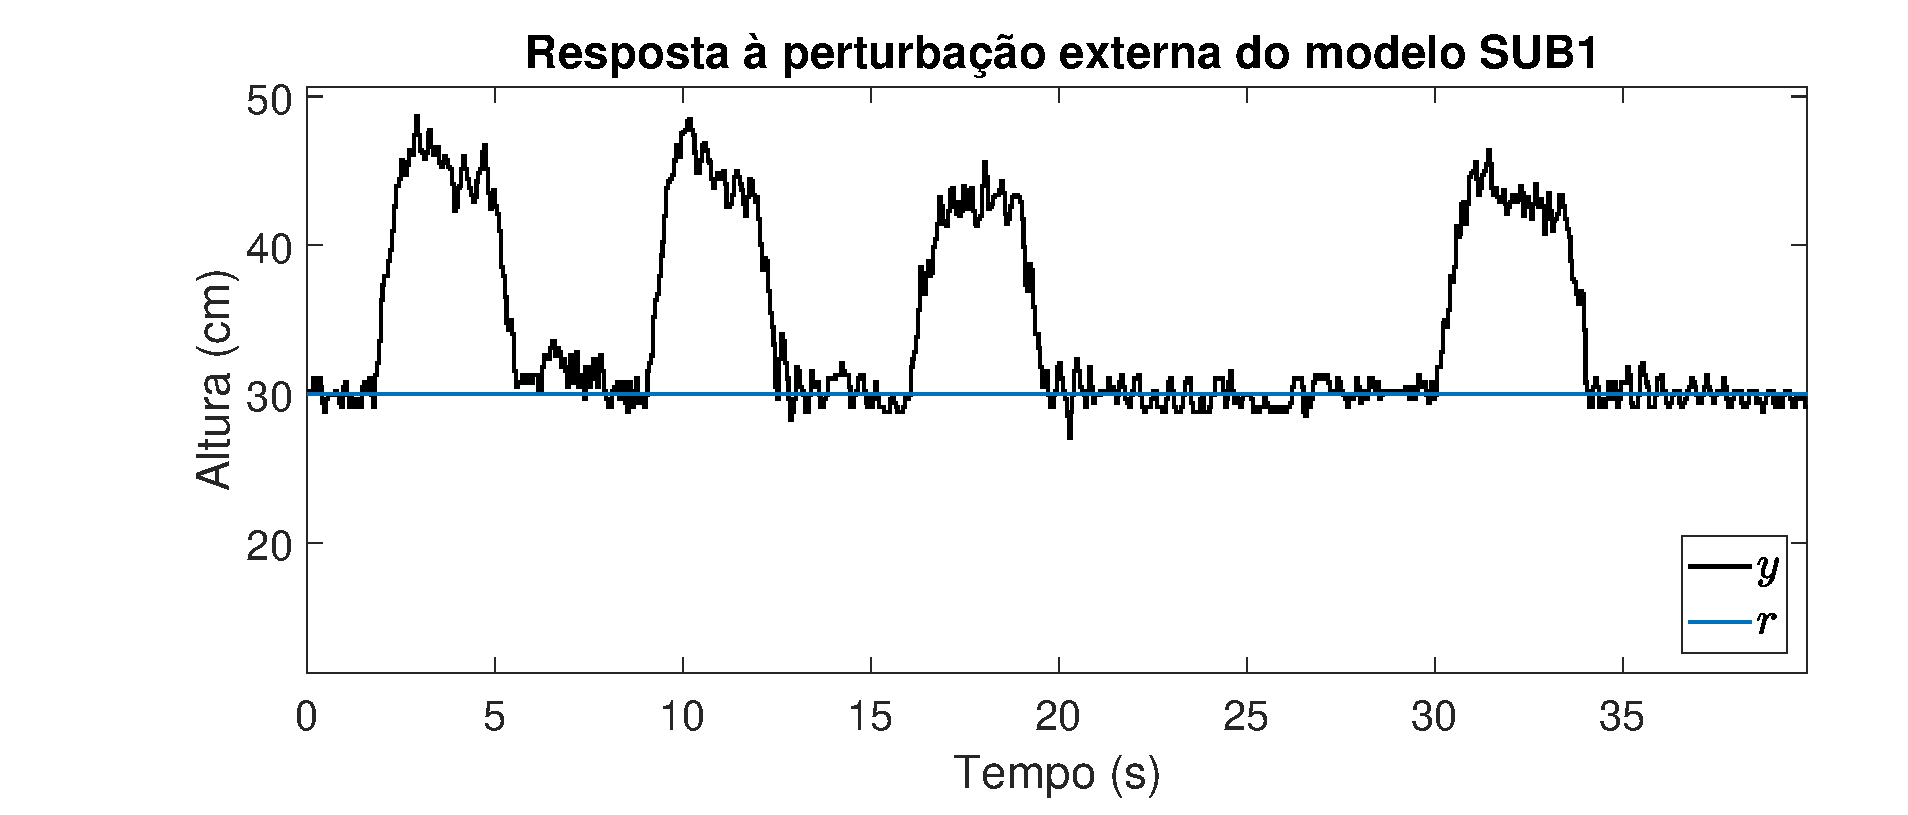
\includegraphics[width=1\linewidth]{pextrealsub1}
	\caption[Resposta à perturbação externa do modelo $SUB1$]{Resposta à perturbação externa do sistema com o controlador do modelo $SUB1$}
	\label{fig:pextrealsub1}
\end{figure}

\begin{figure}[H]
	\centering
	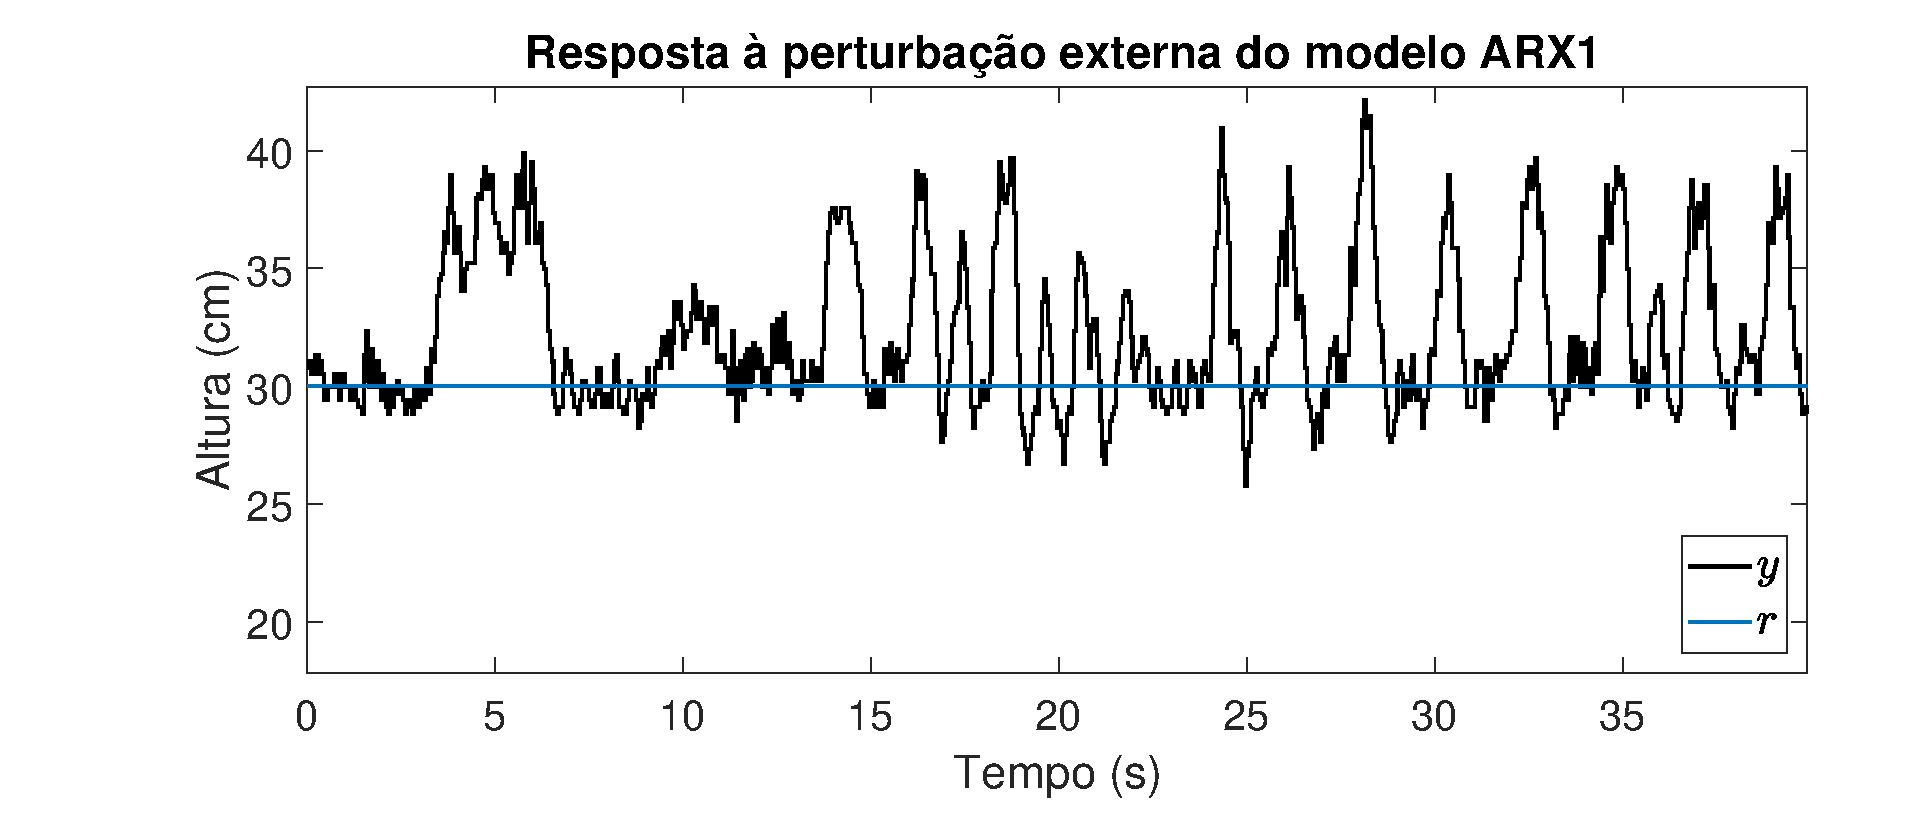
\includegraphics[width=1\linewidth]{pextrealarx1}
	\caption[Resposta à perturbação externa do modelo $ARX1$]{Resposta à perturbação externa do sistema com o controlador do modelo $ARX1$}
	\label{fig:pextrealarx1}
\end{figure}

\begin{figure}[H]
	\centering
	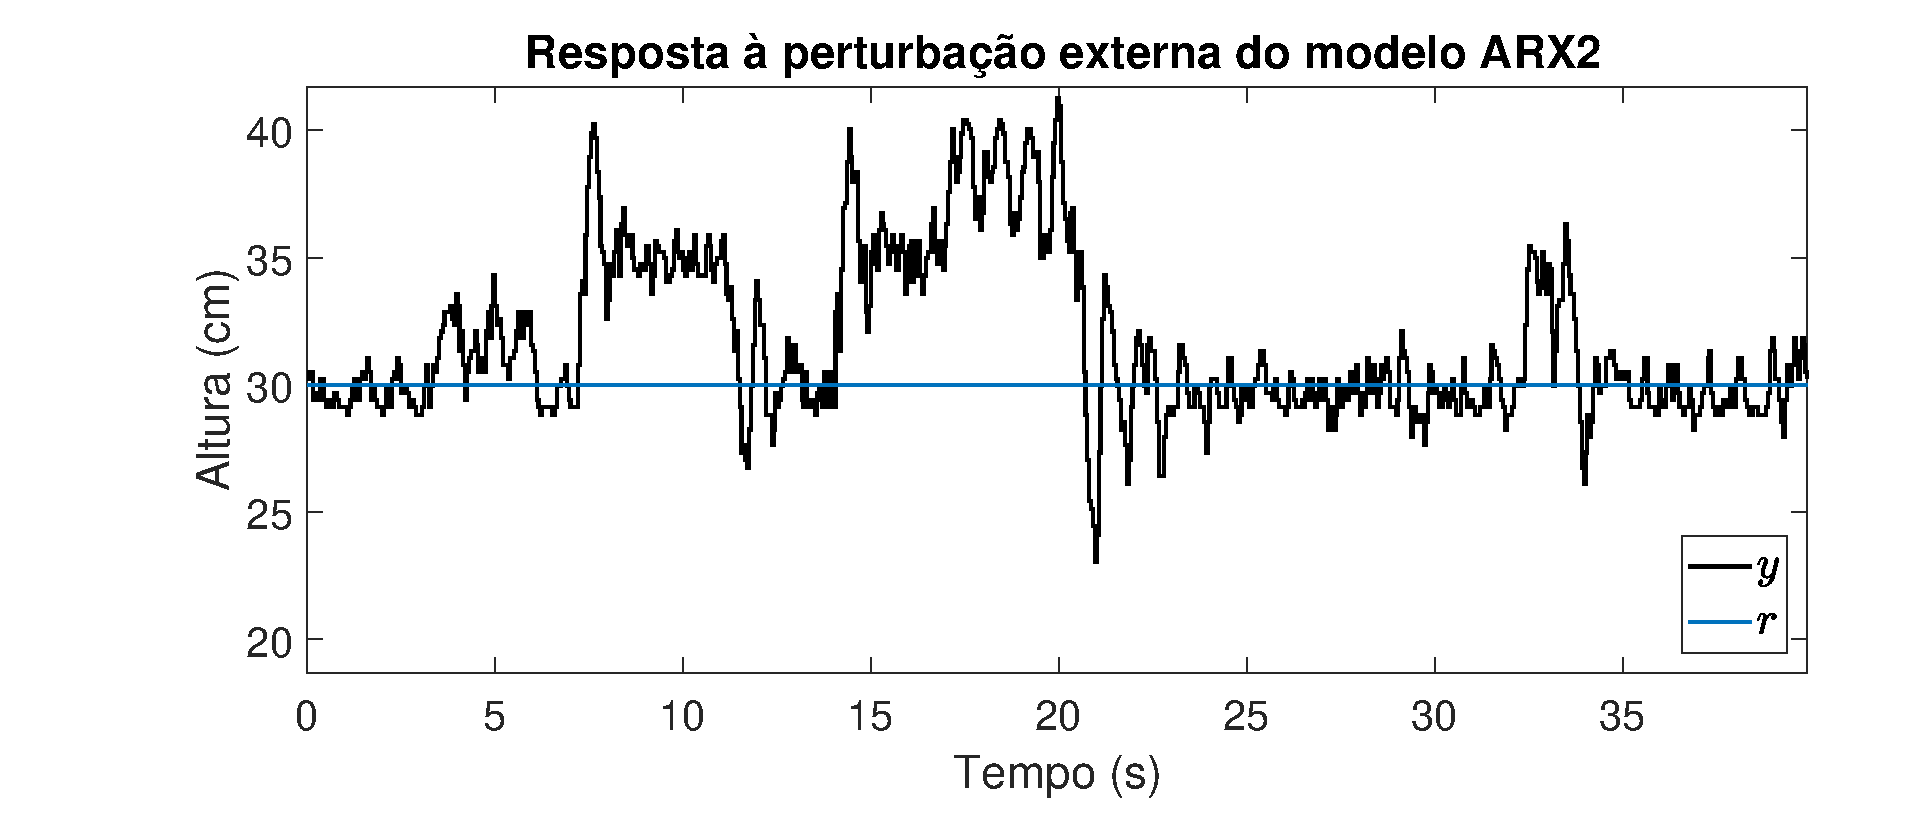
\includegraphics[width=1\linewidth]{pextrealarx2}
	\caption[Resposta à perturbação externa do modelo $ARX2$]{Resposta à perturbação externa do sistema com o controlador do modelo $ARX2$}
	\label{fig:pextrealarx2}
\end{figure}



\section{Discussão}

Vemos nas figuras da seção \ref{rstep} que os modelos $SUB1$, $ARX1$ e $ARX2$ atendem ao requisito de tempo de assentamento mas não atendem ao requisito de máximo sobrevalor, apesar de que eles não cheguem a estabilizar completamente em um ponto. Isso acontece devido uma série de fatores possíveis, ruído no sensor, reflexo dos raios infra vermelhos na parede do túnel de vento, atuação falha no motor. 


Na seção \ref{rstair} vemos que com o controlador projetado é capaz de fazer o sistema seguir os diferentes níveis de tensão e estabilizar. Para os modelos $ARX1$ e $ARX2$ o sistema se mostra estabilizado enquanto a referência está em 35 cm.


Na seção \ref{rmp} fica claro que nenhum dos controladores projetados tem capacidade para reagir à mudança de parâmetros. 


Na seção \ref{rpe} vemos que nenhum dos controladores rejeita perturbações externas. 








